\documentclass[]{book}

\usepackage{import}
\usepackage{preamble}
\usepackage{tikz}

\begin{document}

\noindent BECA / Huson / 11.1 IB Math SL \hspace{2in} Name:\\*
30 October 2017
\begin{center}
{\Large Homework: Exponents and radicals}\\
\textit{Do these problems without a calculator. Answer the first page on loose leaf paper.}
\end{center}

%\vspace{0.2 cm}


Simplify, leaving no negative or fractional exponents.

\begin{enumerate}

\item $\displaystyle 4^{-1}x^{-2} \times \frac{8}{9}x^4 y^{-3}$\\[10pt]
\item $\displaystyle  \frac{x \sqrt{25x^4}}{\sqrt[3]{7x^{-6}}}$\\[10pt]
\item $x^3 y^{-3} \div x^{-4} y^2$\\[10pt]
\item $(-a^2)^2$\\[10pt]

\item $\displaystyle \frac{6}{5} (x^{-2} y)^2 \times \frac{1}{3}(x^4 y^{-1})$\\[10pt]

\item $\displaystyle  125^\frac{4}{3}$\\[10pt]
\item $\displaystyle  (1.21)^{\frac{1}{2}}$\\[10pt]

\item $\displaystyle  36^\frac{1}{4}$\\[10pt]
\item $\displaystyle  \sqrt[3]{\frac{x^6 y^{-12}}{z^{-3}}}$\\[10pt]

\item Let $f(x) = x^2 - 4$.
\begin{enumerate}
    \item Rewrite this function in vertex form and state the vertex as an ordered pair.
    \item $g(x)=f(x+5)+2$. Write $g(x)$ in vertex form.
    \item State the geometric transformation that maps $f$ into $g$.
    \item Find $f^{-1}(x)$
\end{enumerate}

\item Let $f(x) = (x-2)^2 - 3x$ and $g(x)=3x-2$. Find $(f \circ g) (x)$


\newpage 

\item Let $\displaystyle f(x) = (\frac{1}{2})^x$, for $-4 \leq x \leq 4$.
\begin{enumerate}
\item On the  grid below, graph $f$.
\item Write down the value of $f(0)$.
\item Using the graph, solve for $f(x)= \frac{1}{4}$.
\item What is the value of $f^{-1}(8)$?
\end{enumerate}



\begin{figure}[!htbp]
\begin{center}
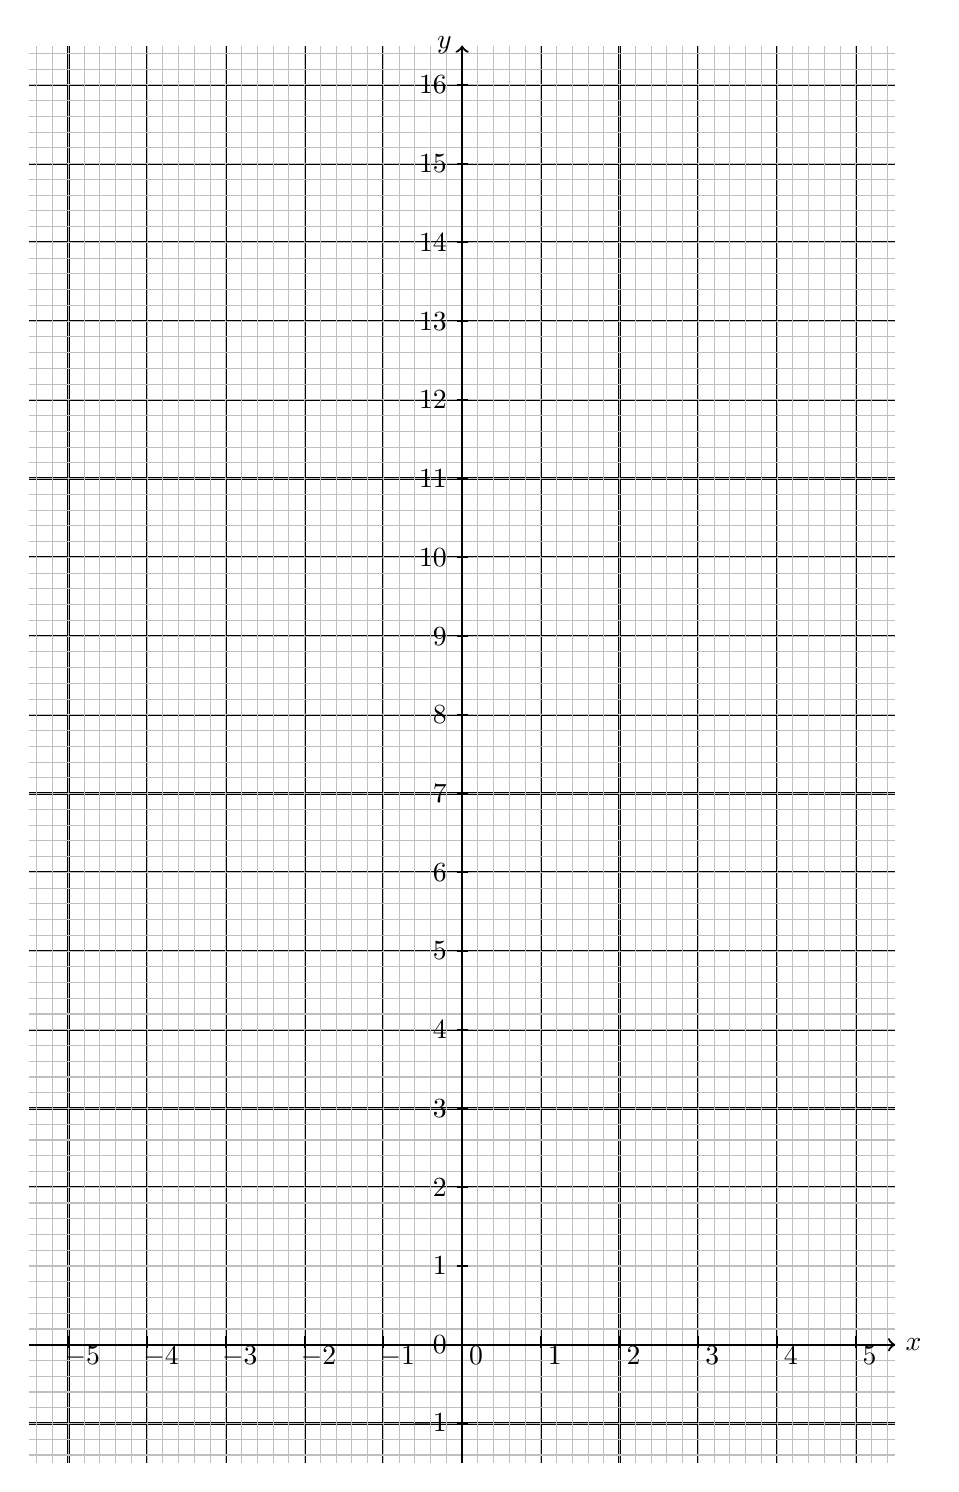
\begin{tikzpicture}

%grid
\draw [thick, color=black,, xstep=1.0cm,ystep=1.0cm] (-5.5,-1.5) grid (5.5,16.5);
\draw [thin, color=lightgray,, xstep=0.2cm,ystep=0.2cm] (-5.5,-1.5) grid (5.5,16.5);

\foreach \x in {-5, -4, -3, -2, -1, 0,1,2,3,4,5}
\draw[shift={(\x,0)},color=black] (0pt,-1pt) -- (0pt,3pt) node[below]  {$\quad \x$};

\foreach \y in {-1,0,1,2,3,4,5, 6, 7, 8, 9, 10, 11, 12, 13, 14, 15, 16}
\draw[shift={(0,\y)},color=black] (2pt,0pt) -- (-2pt,0pt) node[left]  {$\y$};

\draw [thick, ->] (-5.5,0) -- (+5.5,0) node [right] {$x$};
\draw [thick, ->] (0,-1.5) -- (0,16.5) node [left] {$y$};

\end{tikzpicture}
\end{center}
\end{figure}

\newpage 

\item The function $f(x)=e^x$ is shown on the graph. Sketch $g(x)=f(x-3)$.

\begin{figure}[!htbp]
\begin{center}
\begin{tikzpicture}

%grid
%\draw [thick, color=black,, xstep=1.0cm,ystep=1.0cm] (-5.5,-1.5) grid (5.5,16.5);
%\draw [thin, color=lightgray,, xstep=0.2cm,ystep=0.2cm] (-5.5,-1.5) grid (5.5,16.5);

\foreach \x in {-5, -4, -3, -2, -1, 0,1,2,3,4,5}
\draw[shift={(\x,0)},color=black] (0pt,-3pt) -- (0pt,3pt) node[below]  {$\x$};

\foreach \y in {-1,0,1,2,3,4,5, 6, 7}
\draw[shift={(0,\y)},color=black] (2pt,0pt) -- (-2pt,0pt) node[left]  {$\y$};

\draw [thick, ->] (-5.5,0) -- (+5.5,0) node [right] {$x$};
\draw [thick, ->] (0,-1.0) -- (0,7.5) node [left] {$y$};

\draw [<-, ->] plot[domain= -3:2] (\x, e^\x);

\end{tikzpicture}
\end{center}
\end{figure}

\item The function $f(x)=e^x$ is shown on the graph. Sketch $g(x)=f(-x)+2$. Plot and label the asymptote.

\begin{figure}[!htbp]
\begin{center}
\begin{tikzpicture}

%grid
%\draw [thick, color=black,, xstep=1.0cm,ystep=1.0cm] (-5.5,-1.5) grid (5.5,16.5);
%\draw [thin, color=lightgray,, xstep=0.2cm,ystep=0.2cm] (-5.5,-1.5) grid (5.5,16.5);

\foreach \x in {-5, -4, -3, -2, -1, 0,1,2,3,4,5}
\draw[shift={(\x,0)},color=black] (0pt,-3pt) -- (0pt,3pt) node[below]  {$\x$};

\foreach \y in {-1,0,1,2,3,4,5, 6, 7}
\draw[shift={(0,\y)},color=black] (2pt,0pt) -- (-2pt,0pt) node[left]  {$\y$};

\draw [thick, ->] (-5.5,0) -- (+5.5,0) node [right] {$x$};
\draw [thick, ->] (0,-1.0) -- (0,7.5) node [left] {$y$};

\draw [<-, ->] plot[domain= -3:2] (\x, e^\x);

\end{tikzpicture}
\end{center}
\end{figure}

\newpage
\item Graph the function $f(x) = x^2 - 4$ over the domain $x \geq 0$ on the grid below. 
\begin{enumerate}
    \item Label the $y$-intercept as an ordered pair.
    \item Label the point representing the solution to the equation $f(x)=0$ as an ordered pair.\\*[25pt]
    \item Write down the value of $f^{-1}(-3)$ and label the point $(f^{-1}(-3), -3)$.\\*[25pt]
    \item Graph the inverse function, $f^{-1}(x)$.\\*[15pt]
\end{enumerate}

\begin{figure}[!htbp]
\begin{center}
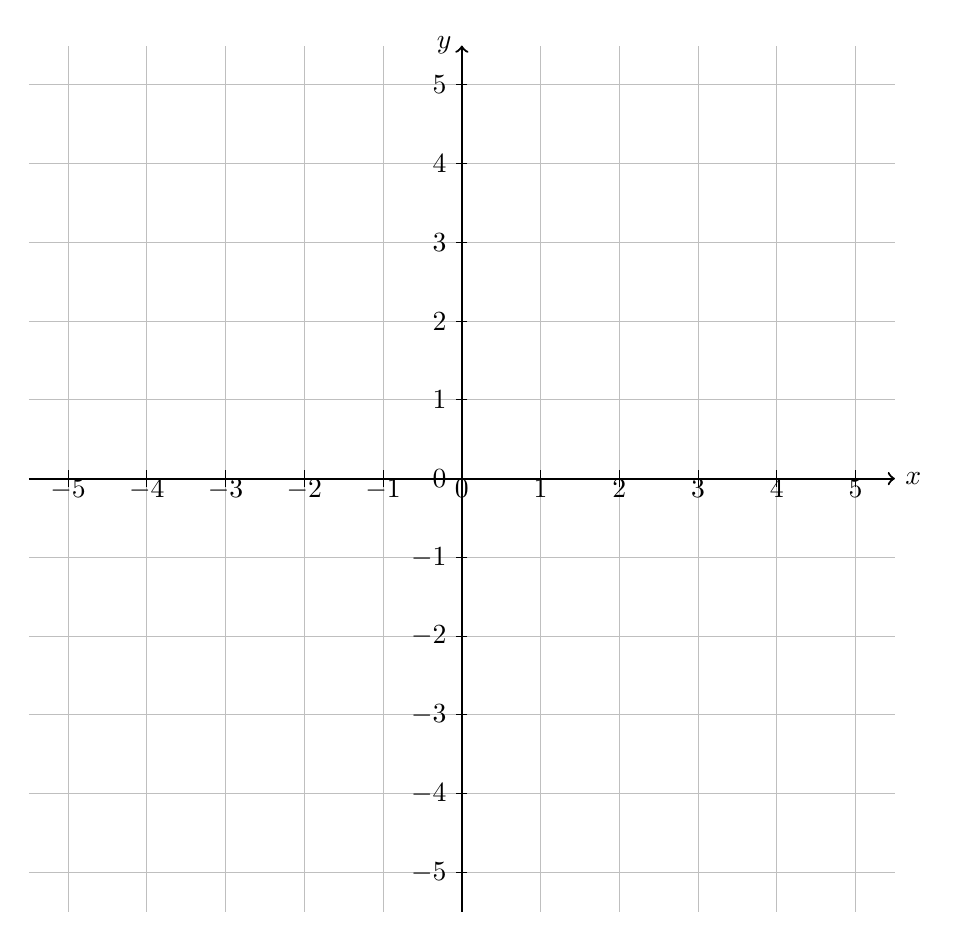
\begin{tikzpicture}

%grid
\draw [thin, color=lightgray,, xstep=1.0cm,ystep=1.0cm] (-5.5,-5.5) grid (5.5,5.5);
%\draw [thin, color=lightgray,, xstep=0.2cm,ystep=0.2cm] (-5.5,-1.5) grid (5.5,16.5);

\foreach \x in {-5, -4, -3, -2, -1, 0,1,2,3,4,5}
\draw[shift={(\x,0)},color=black] (0pt,-3pt) -- (0pt,3pt) node[below]  {$\x$};

\foreach \y in {-5, -4, -3, -2, -1, 0,1,2,3,4,5}
\draw[shift={(0,\y)},color=black] (2pt,0pt) -- (-2pt,0pt) node[left]  {$\y$};

\draw [thick, ->] (-5.5,0) -- (+5.5,0) node [right] {$x$};
\draw [thick, ->] (0,-5.5) -- (0,5.5) node [left] {$y$};

%\draw plot[domain= 0:3] (\x, \x*\x - 4);

\end{tikzpicture}
\end{center}
\end{figure}



\end{enumerate}

\end{document}